\section{Planning with Control Parameters as SMT}\label{sec:control_parameters}

PDDL is known as an expressive modelling language, however it enforces a significant limitation on the modelling of durative actions, restricting the action parameters to choose their values from finite domains. The parameter domains for actions are specified in the problem description, enumerated as a list of objects. Using this enumeration, the action schemes can be grounded, producing a finite set of grounded actions.
%
The only exception to finite domain parameters, introduced in PDDL2.1, is the duration of durative actions. The duration of a durative action can be chosen by the planner. This makes possible the modelling of duration dependent effects. Without the flexible duration parameter, the state space is always locally finite, which is to say that only finitely many states are reachable from a given initial state, using plans bounded by a given finite length. The addition of numeric state variables to the classical propositional language allows for the construction of an infinite state space~\cite{savas2016planning}.

Savas et al.~\cite{savas2016planning} introduces new set of numeric action parameters called \textit{control parameters}: a generalised version of the duration parameter, which allows the planner to choose their values from an infinite domain. The control parameters can appear both in the conditions and the effects of a durative action. Control parameters as described by Savas et al. are constrained with an upper bound and a lower bound in the domain file. The main example used by Savas et al. is a domain which includes the action of withdrawing cash from an ATM (referred to as the \textit{cashpoint} example). Choosing the value of the withdrawal is a numeric control parameter in this action. Without this numeric control parameter the amount of withdrawal would have to be modelled by a set of actions discretising the real-valued parameter, or by introducing actions to increase and decrease the amount of withdrawal by a fixed step size. In either case, the amount of withdrawal is restricted to a discretisation and the number of actions is increased.

In this section we briefly describe how PDDL is extended to include control parameters, and later we show the extension to our SMT encoding for the domains with control parameters. We use the \textit{cashpoint} domain as a running example throughout the section.

\subsection{Cashpoint Problem}

In the cashpoint problem, suppose that we want to go to a pub. Figure~\ref{fig:cashpoint} shows the initial state and goal of the cashpoint problem. Initially we are at home and have \pounds2 in our pocket. The aim of the problem is to be at the pub with \pounds20 in our pocket and have purchased snacks on the way to the pub.

% cashpoint example
\begin{figure}[!ht]
\centering
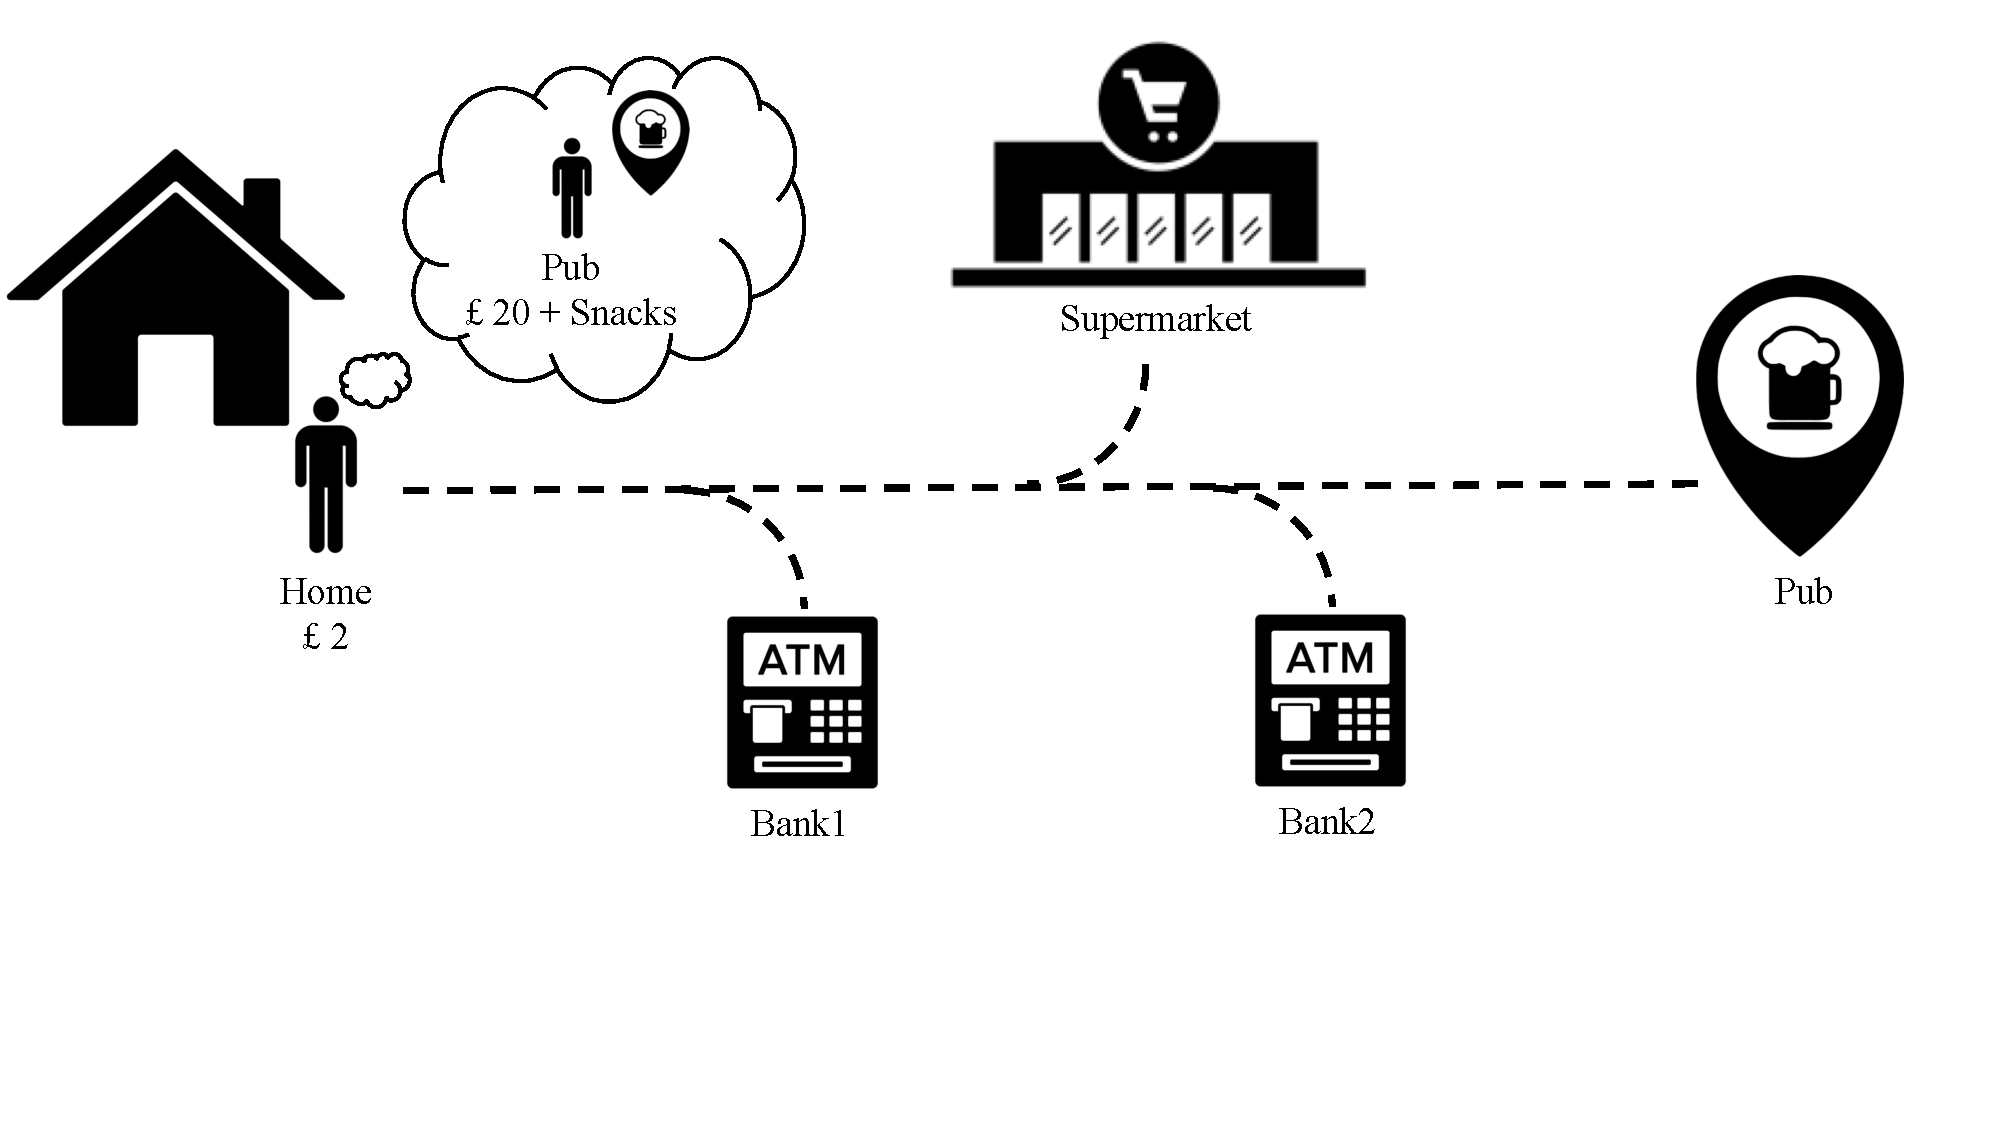
\includegraphics[width=0.80\textwidth]{diagrams/cashpoint.pdf}
\caption{Initial state and goal of the cashpoint problem. The person is initially at home with \pounds2 and the goal is to be at the pub with snacks and \pounds20.}
\label{fig:cashpoint}
\end{figure}

The amount of money that the we withdraw from the cash machine is defined as a control parameter whose value is chosen by the planner. The proposed PDDL domain with control parameters is an extended version of PDDL2.1 in which durative actions can include an additional field for control parameters.

Figure~\ref{fig:actions cashpoint domain} illustrates the domain for this problem. The action $(withdraw\_money)$ is a durative action with the control parameter $(?cash - number)$. In this action, the control parameter is used in the effects of the action and not in the conditions. As the effect of this action, the numeric variable $(inpocket \ \ ?z)$ where $?z$ is the type of currency, is increased by the value of the control parameter. Similar to that the numeric variable $(maxwithdraw \ \ ?b \ \ ?z)$ where $?b$ is the location that we withdraw money from (bank1 or bank2), has been decreased by the same value.

\begin{figure}[thb]
\scriptsize
\begin{verbatim}
(:durative-action withdraw_money
:parameters (?b - location ?z - currency)
:control (?cash - number)
:duration (= ?duration 2)
:condition (and (over all (at ?b)) 
                (at start (>= ?cash 5))
                (at start (<= ?cash 100))
                (at start (>= (maxwithdraw ?b ?z) 0 ))
                (at end (>= (maxwithdraw ?b ?z) 0))
                (at start (available))
                (at start (canwithdraw_money ?b))
				)
:effect (and   	
                (at start (not (available)))
                (at start (increase (inpocket ?z) ?cash))
                (at start (decrease (maxwithdraw ?b ?z) ?cash))
                (at end (available))
        ))

        
(:durative-action buy_snacks
:parameters (?a - location ?z - currency)
:duration (= ?duration 1)
:condition (and     (at start (at ?a))
                    (over all (at ?a))
                    (at start (available))
                    (at start (>= (inpocket ?z) 5))
                    (at end (>= (inpocket ?z) 0))
                    (at start (canbuy ?a ?z)) )
:effect (and    (at start (decrease (inpocket ?z) 5)) 
                (at start (not (available)))
                (at end (gotsnacks))
                (at end (available))
        ))
        
(:durative-action check_pocket
:parameters (?z - currency)
:duration (<= ?duration 0.5)
:condition (and     (at start (>= (inpocket ?z) 100) )
                    (at start (available))
                    (at end (>= (inpocket ?z) 0) )  )
:effect (and        
                    (at start (not (available)))
                    (at end (have_enough ?z)) 
                    (at start (decrease (inpocket ?z) 100))
                    (at end (available)) ) )      

) 
\end{verbatim}
\caption{Main actions of the cashpoint domain}
\label{fig:actions cashpoint domain}
\end{figure}

Figure~\ref{fig:cashpoint problem} shows an example problem file for the cashpoint domain. In the problem file for this example there are five locations. Two banks, each of which has a maximum amount of \pounds200 to withdraw, a supermarket where snacks can be purchased, the pub, and the home. Later, we use this example to show the encoding of control parameters.

\begin{figure}[thb]
\scriptsize
\begin{verbatim}
   (:objects pub supermarket home - location
           bank1 bank2 - location
           pounds - currency)
 
   (:init (at  home)
        (canbuy supermarket pounds)
        (canwithdraw_money bank1)
 		(available)
        (= (maxwithdraw bank1 pounds) 200)
        (= (maxwithdraw bank2 pounds) 200)
        (= (inpocket pounds) 2)
 )
		
 (:goal (and (have_enough pounds) (gotsnacks) (at pub) (>= (inpocket pounds) 20) ))
)      
\end{verbatim}
\caption{An example problem file for the cashpoint domain.}
\label{fig:cashpoint problem}
\end{figure}

\subsection{Encoding of PDDL Domains with Control Parameters}

In this section we describe in detail how we extend our previous encoding described in Section~\ref{sec:enc} to handle actions with control parameters. First, we discuss the modifications over the definition of a single happening by introducing control parameters and later we extend these changes to the constraints between happenings.

Following Savas et al.~\cite{savas2016planning}, control parameters are only defined for durative actions. An action with a control parameter, $a\in A$, is defined as:
$$
a := \langle pre_a, eff_a, dur_a, cparam_a \rangle
$$
where $cparam_a$ represents a finite set of numeric control parameters, where each $d^a \in cparam_a$ has a domain $dom(d^a)$. In order to use the control parameters in our encoding, we add a new set of variables to the encoding of a happening explained in Section~\ref{sec:enc_happening}:
$$
D_t := \{ d^a_t \in cparam_a, \forall a\in A \}
$$
where each $d^a_t\in {\rm I\!R}$ describes the value of a control parameter. The encoding of a happening at time $t$ is therefore defined as the tuple:

$$
x_t:=\Bigg \langle 
\begin{array}{l}
\quad time,P_{0,t},\ldots,P_{B,t},P_{B+1,t}\,V_{0,t},\ldots, V_{B,t},V_{B+1,t}\\
\quad D_t,\,E_{0,t},\ldots,E_{B,t},\,Ps_t,\,A_t,\,flow_{V_t},\,dur_{Ps_t}\\
\end{array}
\Bigg \rangle 
$$

By introducing the control parameter variables, the constraints over a happening are extended in the following way. As explained before, the control parameters are bounded in the domain file. First, two sets are defined $U_d$ and $L_d$. The members of set $U_d$ are constants which define the upper bounds of control parameters at each happening (since these upper bounds will not change in different happenings, we do not need to define different upper bounds for each happening). $L_d$ represents the set of lower bounds for the control parameters. Figure~\ref{eq:state2} shows the set of constraints within a happening in the case of having control parameters. The changes are shown in bold compared to Figure~\ref{eq:state}.

\begin{figure*}[thb!]
% \begin{minipage}[t]{0.58\linewidth}
\textbf{Proposition and real variable support}
\begin{enumerate}[label=H\arabic*.]
 % Literal support
  \item $\bigwedge_{p \in P} p_{1,t} \rightarrow (p_{0,t} \vee \bigvee_{e \in E | p \in eff^{+}_{e}} e_{0,t} \vee \bigvee_{a_t \in A | p \in eff^{+}_{a}} a_t)$
  \item $\bigwedge_{p \in P} \neg p_{1,t} \rightarrow (\neg p_{0,t} \vee \bigvee_{e \in E | p \in eff^{-}_{e}} e_{0,t} \vee \bigvee_{a \in A | p \in eff^{-}_{a}} a_t)$
  \item $\bigwedge_{i=1}^{B} \bigwedge_{p \in P} p_{i+1,t}      \rightarrow (     p_{i,t} \vee \bigvee_{e \in E | p \in eff^{+}_{e}} e_{i,t})$
  \item $\bigwedge_{i=1}^{B} \bigwedge_{p \in P} \neg p_{i+1,t} \rightarrow (\neg p_{i,t} \vee \bigvee_{e \in E | p \in eff^{-}_{e}} e_{i,t})$
 % Real variable support
  \item $\bigwedge_{v \in V} (\bigwedge_{a \in A | v \in eff^{num}_{a}} \neg a_{t} \wedge \bigwedge_{e \in E | v \in eff^{num}_{e}} \neg e_{0,t}) \rightarrow (v_{i+1,t} = v_{i,t})$
  \item $\bigwedge_{i=1}^{B} \bigwedge_{v \in V} (\bigwedge_{e \in E | v \in eff^{num}_{e}} \neg e_{i,t}) \rightarrow (v_{i+1,t} = v_{i,t})$
\end{enumerate}
\textbf{Event preconditions and effects}
\begin{enumerate}[label=H\arabic*.]\setcounter{enumi}{6}
 % event preconditions
 \item $\bigwedge_{i=0}^{B} \bigwedge_{e \in E} e_{i,t} \leftrightarrow pre_{e} (P_{i} \cup V_{i})$
 % event effects
 \item $\bigwedge_{i=0}^{B} \bigwedge_{e \in E} e_{i,t} \rightarrow eff_{e} (P_{i+1} \cup V_{i+1})$
\end{enumerate}
% \end{minipage}
% \begin{minipage}[t]{0.42\linewidth}
\textbf{{Action preconditions and effects}
\begin{enumerate}[label=H\arabic*.]\setcounter{enumi}{8}
 % Action preconditions
 \item \bm{$\bigwedge_{a \in A} a_t \rightarrow pre_{a}(P_{0,t} \cup V_{0,t})$}
  % action effects
 \item \bm{$\bigwedge_{a \in A} a_t \rightarrow eff_{a}(P_{1,t} \cup V_{1,t})$}
\end{enumerate}}
%\textbf{Support across epsilon separation}
%\begin{enumerate}[label=H\arabic*.]\setcounter{enumi}{10}
 % literal support
% \item $\bigwedge_{p_{B+1,t}\in P} p_{B+1,t} \rightarrow p_{B,t}$
% \item $\bigwedge_{p_{B+1,t}\in P} \neg p_{B+1,t}\rightarrow \neg p_{B,t}$
%\end{enumerate}
\textbf{Process triggering}
\begin{enumerate}[label=H\arabic*.]\setcounter{enumi}{10}
 % process triggering
 \item $\bigwedge_{ps\in Ps} ps_t \leftrightarrow pre_{ps}(P_{B+1,t} \cup V_{B+1,t})$
 \item $\bigwedge_{ps\in Ps} dur_{ps_t} >= 0$
 \item $\bigwedge_{ps\in Ps} ps_t \leftrightarrow (dur_{ps_t} > 0)$
\end{enumerate}
\textbf{Action mutexes}
\begin{enumerate}[label=H\arabic*.]\setcounter{enumi}{13}
 % Action mutexes
 \item $\bigwedge_{a \in A} \bigwedge_{a' \in A | a \nparallel a'} (\neg a_t \vee \neg a'_t)$
\end{enumerate}
% Bounds on control parameters
\textbf{{Bounds on control parameters}
\begin{enumerate}[label=H\arabic*.] \setcounter{enumi}{14} 
\item \bm{$\bigwedge_{d^a_t \in D_t} a_t \rightarrow {d^a_t <= u_d}$}
\item \bm{$\bigwedge_{d^a_t \in D_t} a_t \rightarrow {d^a_t >= l_d}$}
%\item \bm{$\bigwedge_{{a_t\in A}| d^a_t \in \mathit{cparam_a}} a_t \rightarrow {d^a_t <= u_d \in U_d}$ \quad \forall  ${d^a_t\in cparam_a}$}
%\item \bm{$\bigwedge_{{a_t\in A}| d^a_t \in \mathit{cparam_a}} a_t \rightarrow{d^a_t >= l_d \in L_d}$ \quad \forall  ${d^a_t\in cparam_a}$}
\end{enumerate}}
% \end{minipage}
\caption{Reduction of a PDDL+ happening with control parameters to SMT.}
\label{eq:state2}
\end{figure*}

Within a happening, the structure of most of the constraints remain the same. However we need to add the constraints associated with the lower and upper bounds of control parameters (shown in equations $H15$ and $H16$). These constraints state that when the action is applied, the control parameter is bounded by its constant upper and lower bounds $u_d\in U_d$ and $l_d \in L_d$, respectively. In addition, control parameters can appear in the conditions or effect of a durative action. Therefore $H9$ and $H10$ are also affected by control parameters. The control parameter variables $d_t\in D_t$ can be used directly in these constraints.

Adding control parameters to durative actions also affects the encoding of the constraints between the happenings explained in section~\ref{sec:enc_problem}. Figure~\ref{eq:plan2} shows these equations. The changes compared to Figure~\ref{eq:plan} are shown in bold.
The only constraint added to the set of constraints between the happenings is \textit{control parameter support} constraint ($P12$). This constraint ensures that the value of a control parameter stays constant during the execution of the action. In P12, $dur_{ps^a_i}$ refers to the duration variable of the action $a$ containing the control parameter.

\begin{figure*}[thb!]
\begin{minipage}[t]{0.39\linewidth}
\textbf{Instance description}
\begin{enumerate}[label=P\arabic*.]
  % Known states
  \item $I(P_{0,1}\cup V_{0,1})$
  \item $G(P_{B+1,n}\cup V_{B+1,n})$
  % Timing of happenings
  \item $time_0 = 0$
  \item $\bigwedge_{i=2}^n time_i \geq time_{i-1}+\epsilon$
\end{enumerate}
\textbf{Proposition support}
\begin{enumerate}[label=P\arabic*.]\setcounter{enumi}{4}
  % Literal support
  \item $\bigwedge_{i=2}^n \bigwedge_{p\in P} p_{0,i} \rightarrow p_{B+1,i-1}$
  \item $\bigwedge_{i=2}^n \bigwedge_{p\in P} \neg p_{0,i} \rightarrow \neg p_{B+1,i-1}$
\end{enumerate}
\end{minipage}
\begin{minipage}[t]{0.6\linewidth}
\textbf{Invariants}
\begin{enumerate}[label=P\arabic*.]\setcounter{enumi}{6}
  % Process timing conditions (these are necessary in combination to ensure happenings occur at dur=0)
  \item $\bigwedge_{i=2}^n \bigwedge_{ps\in Ps} ps_{i-1} \rightarrow dur_{ps_i} = dur_{ps_{i-1}} - time_i + time_{i-1}$
  % Interval constraints
  \item $\bigwedge_{i=1}^{n-1} \bigwedge_{ps \in Ps}  ps_i \leftrightarrow pre_{\leftrightarrow ps_i}$
  \item $\bigwedge_{i=1}^{n-1} \bigwedge_{e\in E} \neg pre_{\leftrightarrow e_i}$
\end{enumerate}
\textbf{Continuous change on real variables}
\begin{enumerate}[label=P\arabic*.]\setcounter{enumi}{9}
 % Vector flows
  \item $\bigwedge_{i=1}^{n-1} \bigwedge_{v\in V} flow_{v_i} = \int^{time_{i+1}}_{time_i} \sum_{ps\in Ps} eff^{num}_{\leftrightarrow ps}(V_i)dt$
  \item $\bigwedge_{i=2}^n \bigwedge_{v\in V} (v_{0,i} = v_{B+1,i-1} + flow_{v,i-1})$
\end{enumerate}
\end{minipage}
\vspace{1em}\\\textbf{Control parameter support}
\begin{enumerate}[label=P\arabic*.]\setcounter{enumi}{11}
 % control parameter
 \item \bm{$\bigwedge_{i=1}^{n-1} \bigwedge_{d^a_t \in D_t} (dur_{a_i}>0)  \rightarrow (d^a_i = d^a_{i+1})$}
\end{enumerate}
\caption{Reduction of PDDL+ planning problem with control parameters $\Pi+$ to SMT.}
\label{eq:plan2}
\end{figure*}

\subsection{Encoding of the cashpoint problem}

Considering the domain shown above, we introduce a variable $cp\_cash_t$ for each happening as the control parameter associated with the durative action. In this domain we only have one durative action with control parameter:
$$
(withdraw\_money \ \  bank1 \ \  pounds)
$$
The numeric variables associated with this action $(maxwithdraw \ \ \ bank1 \ \ \ pounds)$ and  $(inpocket \ \ \ pounds)$ are affected by the control parameter variable. Constraint $H10$ is modelled as the following constraint, which illustrates the effect of the control parameters on the numeric variables.
$$
\begin{array}{c}
(withdraw\_money\ bank1\ pounds)_{sta,t}  \rightarrow \\
(maxwithdraw\ bank1\ pounds)_{1,t} = ((maxwithdraw\ bank1\ pounds)_{0,t} - cp\_cash_0) \\
\wedge \\
(withdraw\_money\ bank1\ pounds)_{sta,t}  \rightarrow \\
(inpocket\ pounds)_{1,t} = ((inpocket\ pounds)_{0,t} + cp\_cash_0) \\
\end{array}
$$
The upper bound $u_d$ is 100 and the lower bound $l_d$ is 5. Using these bounds we can write the equations $H15$ and $H16$ as :
$$
\begin{array}{l}
(withdraw\_money \, bank1 \, pounds)_{sta,t}  \rightarrow (cp\_cash_0) >=  5 \\
(withdraw\_money \, bank1 \, pounds)_{sta,t}  \rightarrow (cp\_cash_0) <=  25  \\
\end{array}
$$

The plan found by the SMTPlan for this domain and problem file is shown in Figure~\ref{fig:cashpoint plan}. The reason that the planner suggests to withdraw \pounds99.5, is that the action $check\_pocket$ has a precondition $(inpocket \ \ ?z) >= 100$ and the initial value for $(inpocket \ \ pounds)$ is 2. The solution found by the SMT solver is not guaranteed to be optimal with respect to time. This is demonstrated by the plan shown in Figure~\ref{fig:cashpoint plan}, in which there is a 2-second gap between the end of the first withdraw action and the beginning of the second. This is because the only constraint is that the two happenings are separated by at least $\epsilon$, and the SMT solver is left to choose any valid value. It is possible to include a metric for the SMT solver to optimise; for example, the time point of the final happening. However, this does not guarantee optimality with respect to plan duration, as increasing the bound on the number of happenings might lead to a solution with shorter duration.

\begin{figure}[thb]
\small
\begin{verbatim}
0.0:	(goto home bank1) [5.0]
7.0:	(withdraw_money bank1 pounds) [2.0] (?cash [24.0])
11.0:	(withdraw_money bank1 pounds) [2.0] (?cash [99.5])
15.0:	(check_pocket pounds) [0.25]
17.25:	(goto bank1 supermarket) [5.0]
24.25:	(buy_snacks supermarket pounds) [1.0]
27.25:	(goto supermarket pub) [5.0]
\end{verbatim}
\caption{The plan found by the SMTPlan for the cashpoint domain}
\label{fig:cashpoint plan}
\end{figure}

Table~\ref{tab:cashpoint} shows part of a satisfying assignment to an encoding of a problem in the cashpoint domain. The assignment corresponds to the plan shown in Figure~\ref{fig:cashpoint plan}, and displays only the second and third happenings. The second happening occurs 7 time units after starting the plan, and the duration of interval between the two happenings 2 time units.

\begin{table}[htb]
\centering
\small
\def\arraystretch{1.1}
\begin{tabular}{|>{$}l<{$} | >{$}l<{$}|}
\hline
x_2 &  x_3 \\
\hline
t_2:=7 & t_3:=9 \\
\hline
\begin{array}{lr}
available_{0,2} :=1 \\
available_{1,2} :=0 \\
\end{array}
&
\begin{array}{lr}
available_{0,3} :=0 \\
available_{1,3} :=1 \\
\end{array}
\\ \hline
\begin{array}{lr}
maxwithdraw_{0,2} :=200 \\
maxwithdraw_{1,2} := 176 \\
inpocket_{0,2} := 0 \\
inpocket_{1,2} := 24 \\
\end{array}
&
\begin{array}{lr}
maxwithdraw_{0,3} := 176 \\
maxwithdraw_{1,3} := 176 \\
inpocket_{0,3} := 24 \\
inpocket_{1,3} := 24 \\
\end{array}
\\ \hline
\begin{array}{lr}
withdraw\_money_1 := 1 \\
\end{array}
&
\begin{array}{lr}
withdraw\_money_2 := 0 \\
\end{array}
\\ \hline
\begin{array}{lr}
withdraw\_money_{sta,2}:= 1 \\
withdraw\_money_{end,2} := 0\\
\end{array}
&
\begin{array}{lr}
withdraw\_money_{sta,2}:= 0 \\
withdraw\_money_{end,2} := 1\\
\end{array}
\\ \hline
\begin{array}{lr}
withdraw\_money_{dur,1} := 2\\

\end{array}
&
\begin{array}{lr}
withdraw\_money_{dur,2} :=0\\
\end{array}
\\ \hline
\end{tabular}
\caption{Assignment to numeric and propositional variables associated with the $withdraw\_money$ action in the cashpoint domain. Boolean variables that are true are assigned as 1 and the ones are false are 0.}
\label{tab:cashpoint}
\end{table}
